\documentclass[conference]{IEEEtran}
\usepackage{amsmath, amssymb}
\usepackage{graphicx}
\usepackage{booktabs}
\usepackage{hyperref}
\usepackage{tikz}
\usetikzlibrary{positioning,arrows.meta,shapes.multipart,fit,calc}

% 図の検索パス
\graphicspath{{figs/}}

\title{SystemDK with AITL: Physics-Aware Runtime DTCO via PID, FSM, and LLM Integration}

\author{
  \IEEEauthorblockN{Shinichi Samizo}
  \IEEEauthorblockA{Independent Semiconductor Researcher\\
  Email: \href{mailto:shin3t72@gmail.com}{shin3t72@gmail.com}}
}

\begin{document}
\maketitle

\begin{abstract}
This paper presents SystemDK with AITL, a framework that extends conventional Design-Technology Co-Optimization (DTCO) by embedding control-theoretic loops directly into EDA flows. Compact PID controllers and FSM supervisors stabilize runtime variations (RC delay, thermal coupling, EMI/EMC disturbances). Future extensions (AITL Next) integrate LLM analyzers for adaptive PID retuning and FSM rule regeneration. The framework incorporates FEM analysis and S-parameter measurements into synthesis, P\&R, and STA, ensuring physics-aware closure. Simulations demonstrate order-of-magnitude improvements in timing stability, thermal robustness, and jitter suppression.
\end{abstract}

\section{Introduction}
Scaling to sub-2nm nodes and CFET integration introduces critical runtime effects:
\begin{itemize}
  \item RC delay variation due to interconnect scaling,
  \item Vertical thermal coupling in 3D-ICs,
  \item Stress-induced $V_{th}$ shifts,
  \item EMI/EMC noise degrading jitter and reliability.
\end{itemize}
Traditional DTCO applies static guardbands, leading to inefficiency. SystemDK with AITL proposes embedding runtime control (PID+FSM) and, in the future, LLM-based adaptation.

\section{Proposed Framework}
\subsection{AITL Base}
PID compensates delay/thermal/voltage variations; FSM supervises modes and safety thresholds.
\subsection{AITL Next}
LLM (lightweight, future) analyzes EDA logs, retunes PID gains $(K_p, K_i, K_d)$, and regenerates FSM rules.

\begin{figure}[t]
  \centering
  \resizebox{\columnwidth}{!}{%
  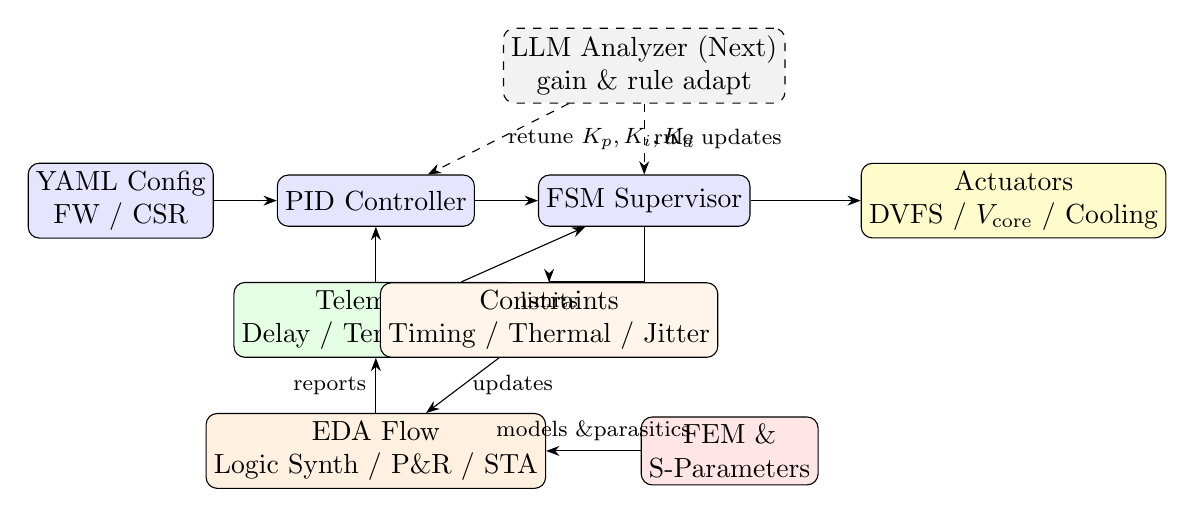
\begin{tikzpicture}[
      node distance=7mm and 8mm,
      box/.style={draw, rounded corners, align=center, inner sep=2.8pt, minimum height=6.5mm},
      ctl/.style={box, fill=blue!10},
      tel/.style={box, fill=green!10},
      eda/.style={box, fill=orange!12},
      phy/.style={box, fill=red!10},
      act/.style={box, fill=yellow!20},
      llm/.style={box, fill=gray!10, dashed},
      lab/.style={font=\footnotesize},
      >=Stealth
    ]

    % --- Control layer ---
    \node[ctl] (yaml) {YAML Config\\FW / CSR};
    \node[ctl, right=of yaml] (pid) {PID Controller};
    \node[ctl, right=of pid] (fsm) {FSM Supervisor};

    % --- Telemetry ---
    \node[tel, below=of pid] (tm) {Telemetry\\Delay / Temp / Jitter};

    % --- EDA flow ---
    \node[eda, below=of tm] (eda) {EDA Flow\\Logic Synth / P\&R / STA};

    % --- Physics inputs ---
    \node[phy, right=12mm of eda] (fem) {FEM \&\\S-Parameters};

    % --- Actuators ---
    \node[act, right=14mm of fsm] (act) {Actuators\\DVFS / $V_{\mathrm{core}}$ / Cooling};

    % --- LLM (Next) ---
    \node[llm, above=9mm of fsm] (llm) {LLM Analyzer (Next)\\gain \& rule adapt};

    % --- Constraints ---
    \node[eda, above=of eda, xshift=22mm, fill=orange!8] (cons) {Constraints\\Timing / Thermal / Jitter};

    % ===== Connections =====
    \draw[->] (yaml) -- (pid);
    \draw[->] (pid) -- (fsm);
    \draw[->] (fsm) -- (act);

    \draw[->] (tm) -- (pid);
    \draw[->] (tm) -- (fsm);

    \draw[->] (eda) -- node[lab,left]{reports} (tm);
    \draw[->] (fsm.south) |- ++(0,-7mm) -| node[lab,below]{limits} (cons);
    \draw[->] (cons) -- node[lab,right]{updates} (eda);

    \draw[->] (fem) -- node[lab,above]{models \&\\parasitics} (eda);

    \draw[->, dashed] (llm) -- node[lab,right]{retune $K_p,K_i,K_d$} (pid);
    \draw[->, dashed] (llm) -- node[lab,right]{rule updates} (fsm);

  \end{tikzpicture}%
  }
  \caption{System overview (1-column): PID\,+\,FSM control with runtime telemetry, EDA flow (Synth/P\&R/STA), physics inputs (FEM/S-parameters), actuators, and LLM (Next).}
  \label{fig:system_overview}
\end{figure}

\section{Analytical Models and EDA Mapping}
\subsection{RC Delay Model}
\[
t_{pd}(T,\sigma,f) = R_0 \cdot (1+\alpha_T (T-T_0)+\alpha_\sigma \sigma)\,C(f)+\Delta_{EMI}(f)
\]
Mapped to STA path delay constraints.

\subsection{Thermal Coupling}
\[
C_{th}\frac{dT}{dt} + \frac{T-T_{amb}}{R_{th}} = P_{chip}(t)
\]
Mapped to P\&R thermal placement constraints.

\subsection{Stress-Induced Vth Shift}
\[
\Delta V_{th}(\sigma)=\kappa \cdot \sigma
\]
Mapped to PDK/SPICE parameter updates.

\subsection{EMI Injection}
\[
v_{emi}(t)=A\sin(2\pi f_{emi} t)
\]
Mapped to SI/EMC jitter constraints.

\section{Simulation Results with EDA Implications}
\subsection{RC Delay Compensation}
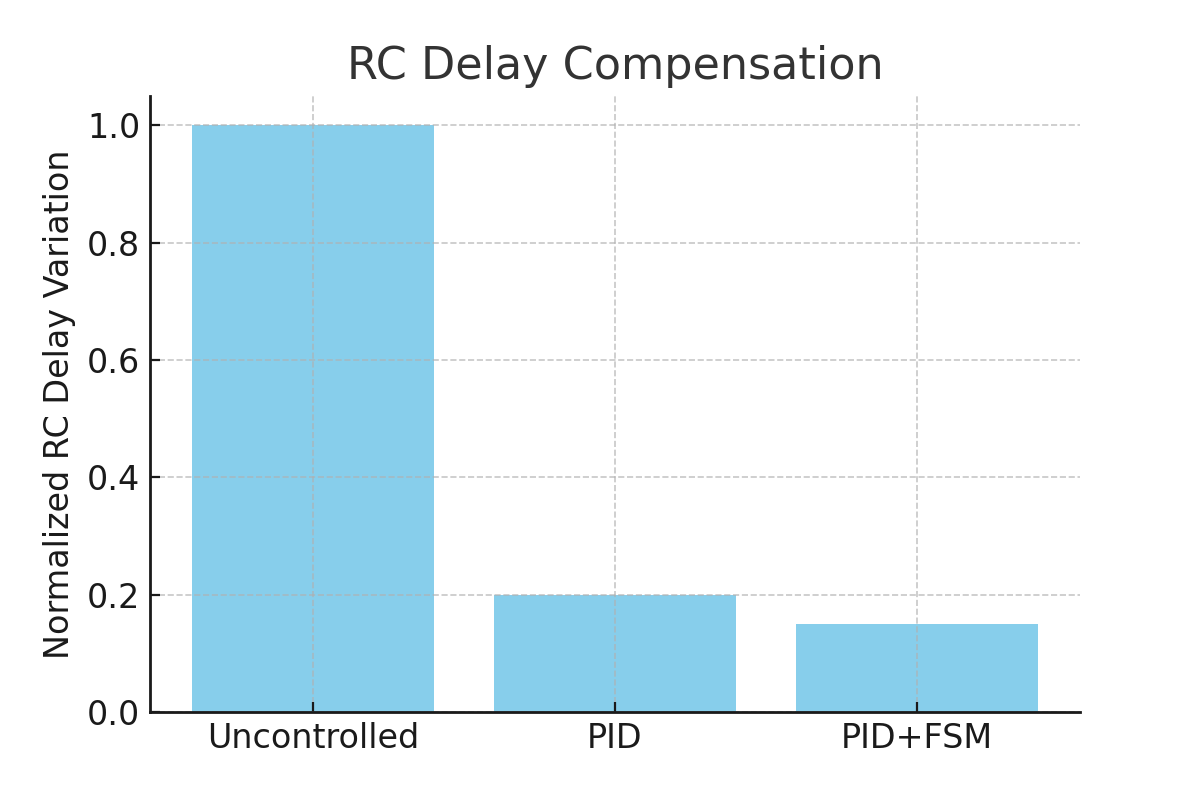
\includegraphics[width=0.45\textwidth]{sim_delay_rc.png}

\subsection{Thermal Response Control}
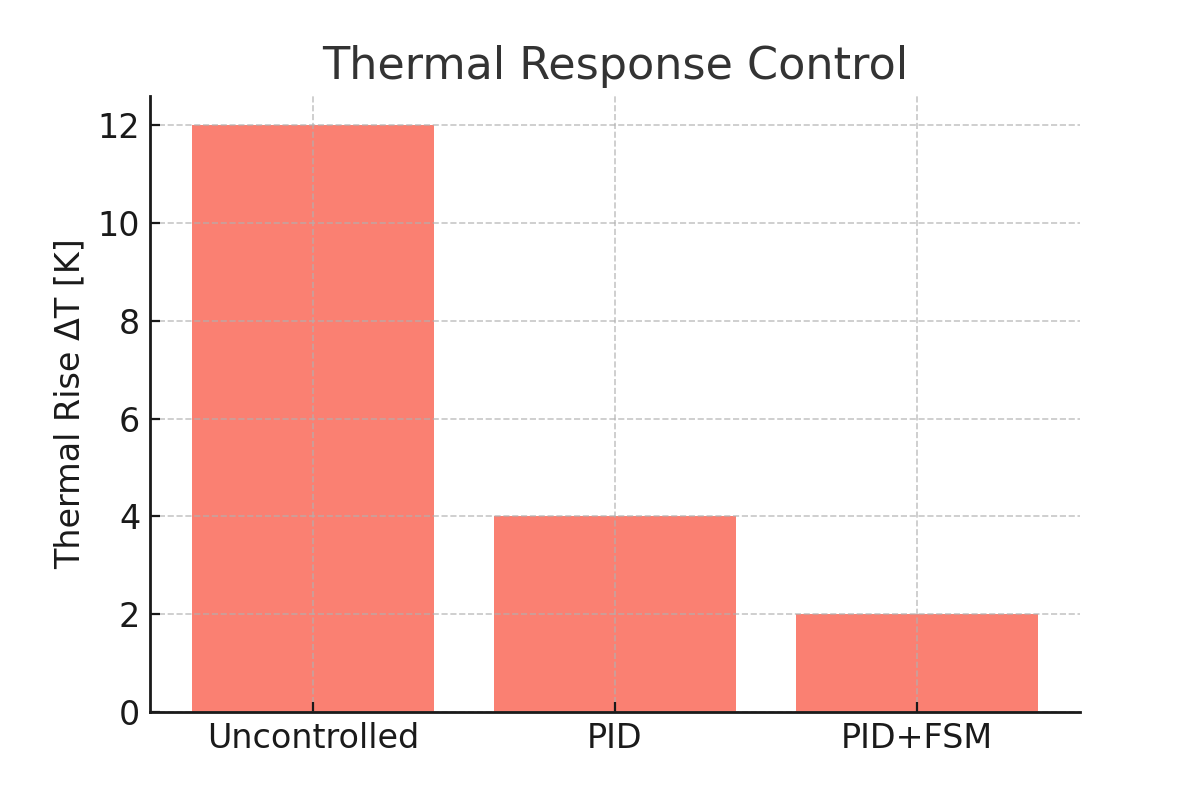
\includegraphics[width=0.45\textwidth]{sim_thermal_response.png}

\subsection{EMI Jitter Suppression}
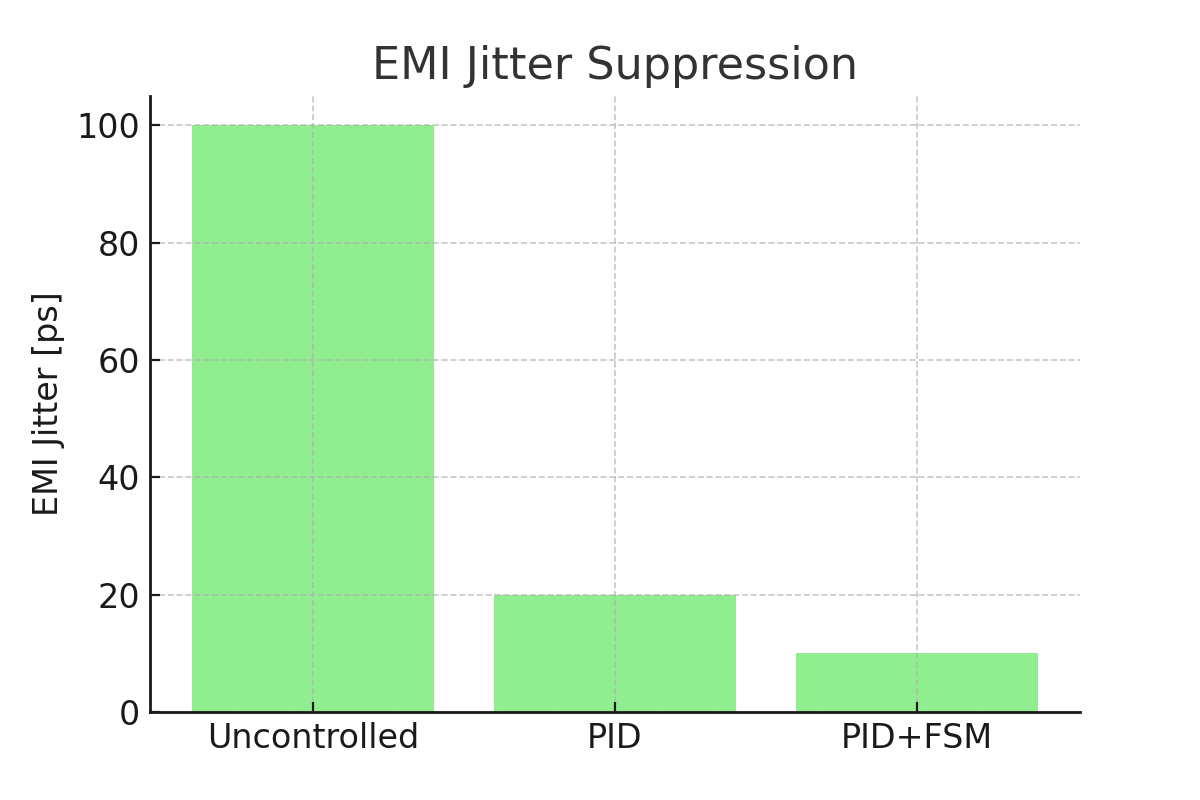
\includegraphics[width=0.45\textwidth]{sim_emi_jitter.png}

\subsection{FEM Analysis}
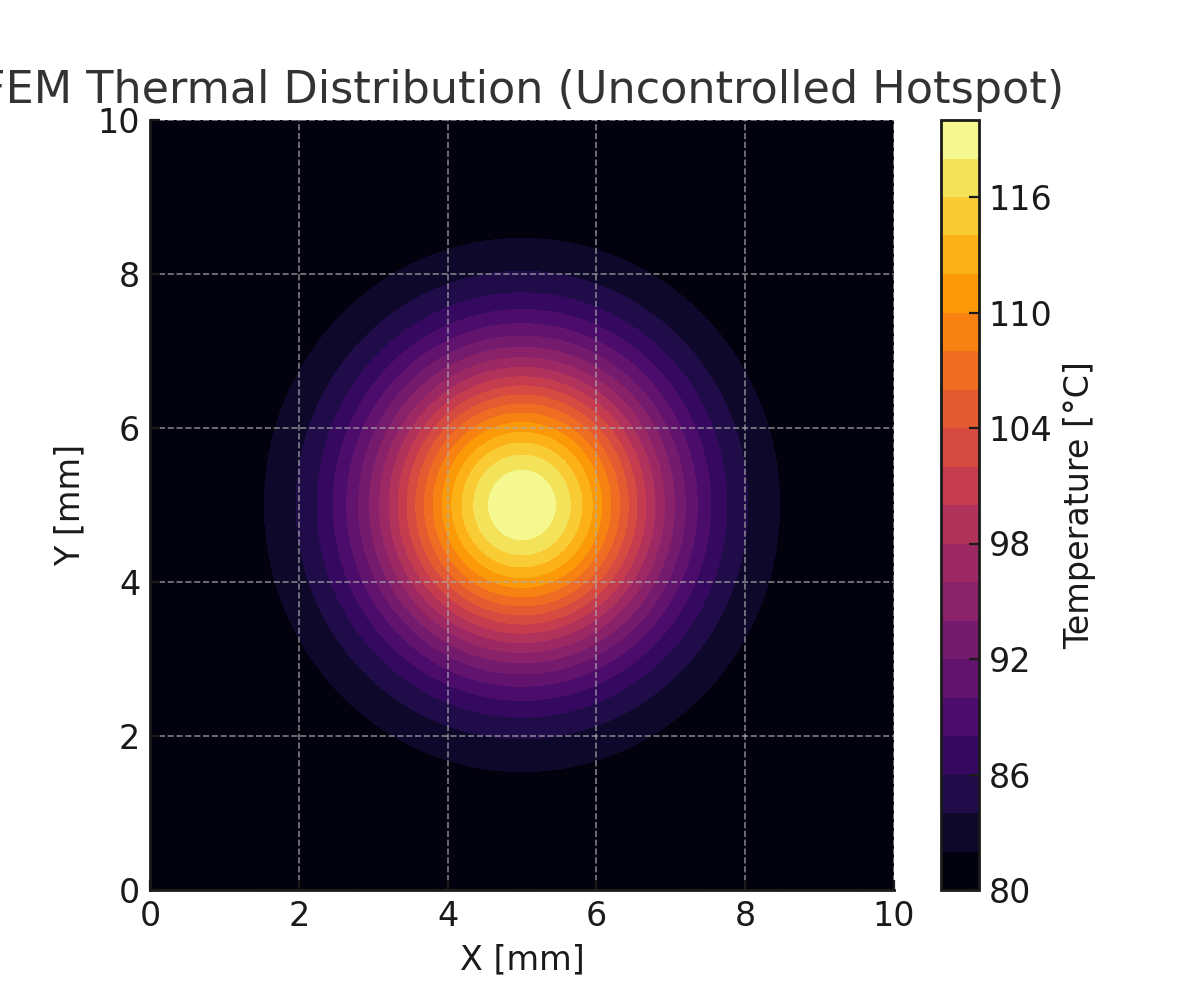
\includegraphics[width=0.45\textwidth]{fem_thermal_map.png}
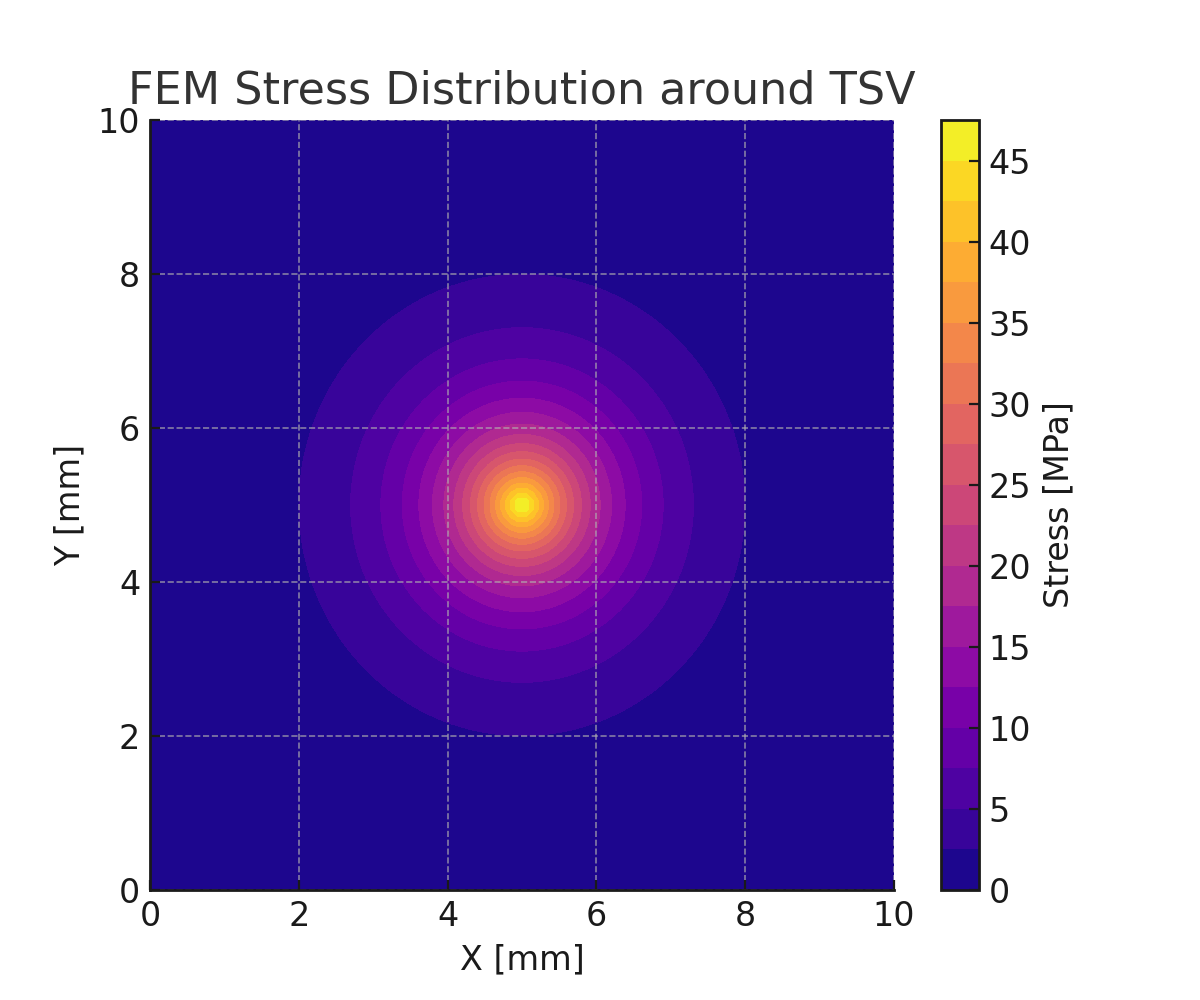
\includegraphics[width=0.45\textwidth]{fem_stress_map.png}

\subsection{S-Parameter Analysis}
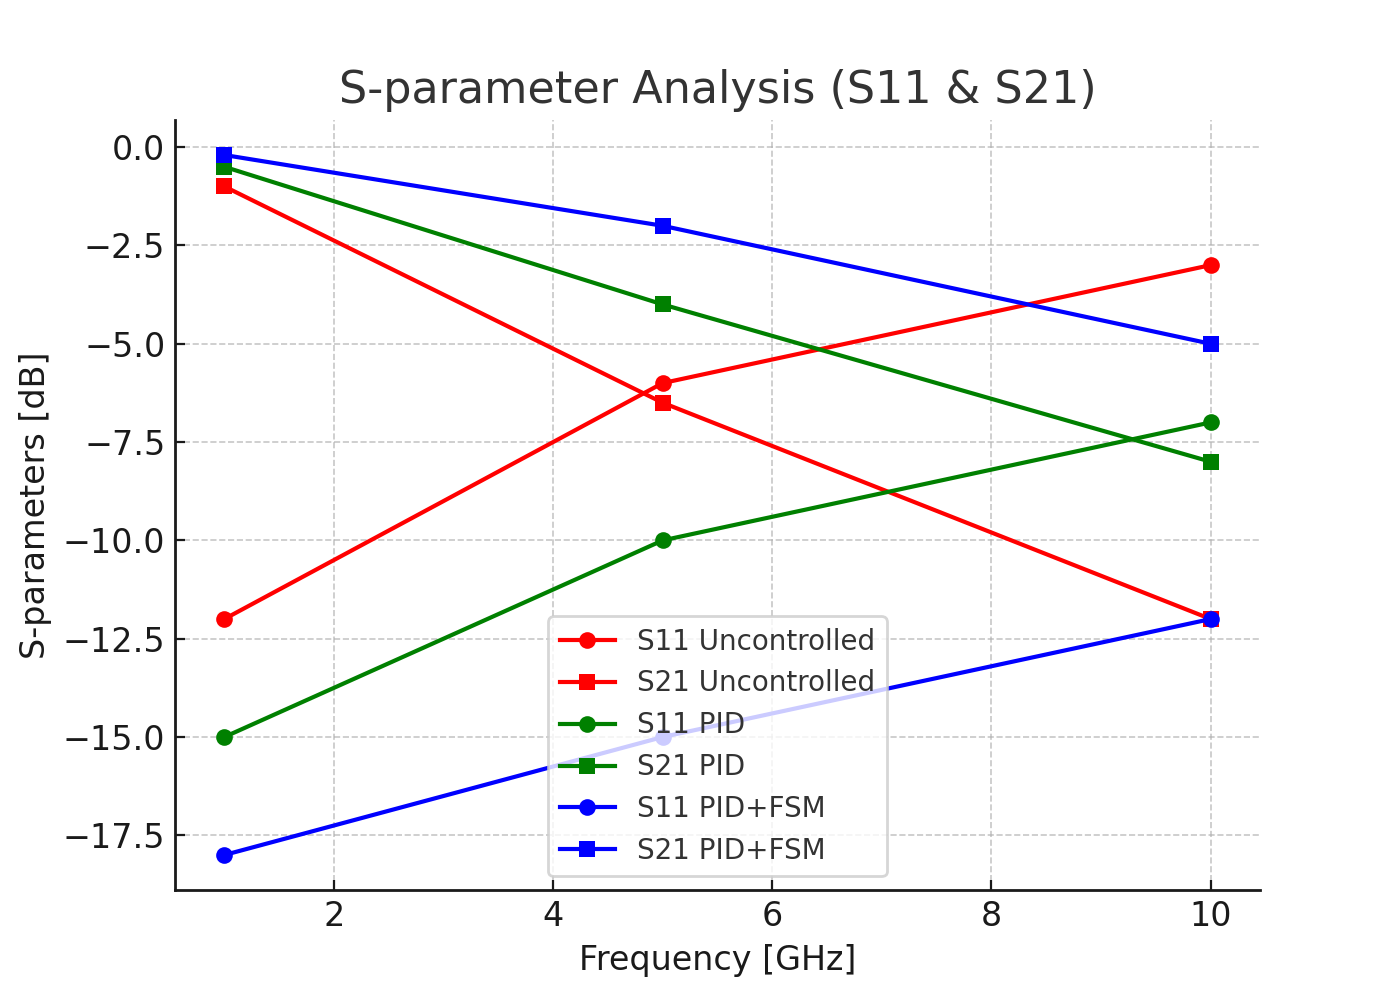
\includegraphics[width=0.48\textwidth]{sparam_s11s21.png}

\section{Implementation PoC}
RTL excerpt (PID controller), FSM transitions, and YAML configuration were implemented in Verilog and integrated with APB/AXI-Lite CSRs.

\section{Discussion}
\begin{itemize}
  \item Guardbands $\to$ adaptive loops,
  \item Static sign-off $\to$ dynamic runtime closure,
  \item Reliability $\to$ cross-domain resilience (delay, thermal, stress, EMI).
\end{itemize}

\section{Conclusion and Future Work}
AITL Base (PID+FSM) establishes runtime stabilization.  
AITL Next will integrate lightweight LLM models for real-time EDA log analysis and control redesign.  
Industrial relevance: prototype chips, EDA tool collaboration, and AI-driven DTCO.

\bibliographystyle{IEEEtran}
\bibliography{systemdk_aitl2025}

\section*{Author Biography}
\noindent\textbf{Shinichi Samizo}
received the M.S. degree in Electrical and Electronic Engineering from Shinshu University, Japan.  
He worked at Seiko Epson Corporation as an engineer in semiconductor memory and mixed-signal device development, and also contributed to inkjet MEMS actuators and PrecisionCore printhead technology.  
He is currently an independent semiconductor researcher focusing on process/device education, memory architecture, and AI system integration.  
\textbf{Contact:} \href{mailto:shin3t72@gmail.com}{shin3t72@gmail.com}, \href{https://github.com/Samizo-AITL}{Samizo-AITL}

\end{document}
